% Capstone Final Project Report
% Spring 2014
% Val Red, Eric Cuiffo, Jeff Adler, Parth Desai, Jeff Rabinowitz
% All rights reserved.

\documentclass[11.5pt,letterpaper,titlepage]{report}


\usepackage[margin=1in]{geometry}

\usepackage{amsmath}
%\bibliographystyle{ieeetr}
\usepackage{graphicx}
\usepackage{subfig}
\usepackage{titling}
\usepackage[utf8]{inputenc}
\usepackage{csquotes}
\usepackage[style=ieee,backend=biber,bibencoding=utf8]{biblatex}
	\addbibresource{citations.bib}
%\usepackage{biblatex-ieee}
%\usepacakge{multicol}
\usepackage[bookmarks=true]{hyperref}
\hypersetup{
    %bookmarks=false,    % show bookmarks bar?
    pdftitle={},    % title
    pdfauthor={},                     % author
    pdfsubject={},        % subject of the document
    pdfkeywords={}, % list of keywords
    colorlinks=true,       % false: boxed links; true: colored links
    linkcolor=blue,       % color of internal links
    citecolor=black,       % color of links to bibliography
    filecolor=black,        % color of file links
    urlcolor=blue,        % color of external links
    linktoc=page            % only page is linked
}%

\usepackage{abbrevs}

\begin{document}
% This inserts the Title, Author, and Date here.
%\maketitle
\begin{titlepage}

\newcommand{\HRule}{\rule{\linewidth}{0.5mm}} % Defines a new command for the horizontal lines, change thickness here


\center % Center everything on the page
 
%----------------------------------------------------------------------------------------
%	HEADING SECTIONS
%----------------------------------------------------------------------------------------

\textsc{\LARGE Rutgers University}\\[1.5cm] % Name of your university/college
\textsc{\Large Capstone Senior Design Project}\\[0.5cm] % Major heading such as course name
\textsc{\large 14:332:492}\\[1.0cm] % Minor heading such as course title

%----------------------------------------------------------------------------------------
%	TITLE SECTION
%----------------------------------------------------------------------------------------

\HRule \\[0.4cm]
{ \huge \bfseries Scarletshield}\\
  \Large A Lightweight, Linux-based Network Security Solution Suite \\[0.4cm] % Title of your document
\HRule \\[3.5cm]
 
%----------------------------------------------------------------------------------------
%	AUTHOR SECTION
%----------------------------------------------------------------------------------------

\begin{minipage}{0.4\textwidth}
\begin{flushleft} \large
\emph{Team:}\\
Jeff \textsc{Adler}\\ % Your name
Eric \textsc{Cuiffo}\\
Parth \textsc{Desai}\\
Jeff \textsc{Rabinowitz}\\
Val A. \textsc{Red}
\end{flushleft}
\end{minipage}
~
\begin{minipage}{0.4\textwidth}
\begin{flushright} \large
\emph{Advisor:} \\
Dr. Manish \textsc{Parashar} % Supervisor's Name
\end{flushright}
\end{minipage}\\[4cm]

% If you don't want a supervisor, uncomment the two lines below and remove the section above
%\Large \emph{Author:}\\
%John \textsc{Smith}\\[3cm] % Your name

%----------------------------------------------------------------------------------------
%	DATE SECTION
%----------------------------------------------------------------------------------------

{\large \today}\\[3cm] % Date, change the \today to a set date if you want to be precise

%----------------------------------------------------------------------------------------
%	LOGO SECTION
%----------------------------------------------------------------------------------------

%\includegraphics{Logo}\\[1cm] % Include a department/university logo - this will require the graphicx package
 
%----------------------------------------------------------------------------------------

\vfill % Fill the rest of the page with whitespace

\end{titlepage}

\tableofcontents
\pagebreak


\newabbrev{\scarletshield}{``Scarletshield''}[Scarletshield]

\newabbrev{\dos}{Denial-of-service (DoS)}[DoS]
\newabbrev{\ddos}{Distributed Denial-of-service (DDoS)}[DDoS]
\newabbrev{\apt}{Advanced Persistent Threat (APT)}[APT]
\newabbrev{\did}{Defense in Depth (DiD)}[DiD]
\newabbrev{\nsa}{National Security Agency (NSA)}[NSA]
\newabbrev{\dns}{Domain Name Service (DNS)}[DNS]
\newabbrev{\ctwo}{Command-and-control (C2)}[C2]
\newabbrev{\distros}{distributions (distros)}[distros]

\chapter{Abstract}

\scarletshield is a customized Ubuntu 12.04 LTS image featuring a uniquely
layered cyber security deployment of several open source services; most notably
the \textbf{''Snort'' Intrusion Detection System (IDS)} utilizing packet inspection and the
\textbf{''Fail2ban'' Intrusion Prevention System (IPS)} utilizing log inspection.  It is
optimized for synergetic network defense and complemented by a dynamic, modern
web frontend providing the utmost flexibility for network administrators to
monitor and quickly react to any and all threats against a network.  The design
of  was conceived as a proof-of-concept to expand upon the more
orthodox but aging \did strategy that layers \emph{overlapping}
technologies rather than presenting varied layers of \emph{complement} defense services
working in \emph{synergy}, which is the approach use to expand upon the defense-in-
depth strategy.  In addition, \scarletshield enables the potential for a user to
interface with interconnected subnets and gateways over a private network to
enable scalability and mitigate large-scale attacks.  Overall, \scarletshield is
intended to be a flexible, open-source system for preventing and thwarting
evolving \ddos Attacks and \apt
by implementing a synergy of various open source and custom
designed services designed to be as flexible and as intuitive as possible for
the network administrator to interface with, minimizing administrative overhead
and maximizing mobility for the network administrator to track and react to
threats.

\section{Introduction}

Attackers have the edge in the dynamically evolving field of cyber security.
With a wider breadth of strategies, near-infinite resources, and a virtually
untraceable mask of anonymity; hackers have long boasted the advantage,
successfully rendering useless the generally accepted \did layered
defense mechanisms most organizations deployed for network defense.
Essentially, is analogous to an onion: although it is deeply
layered, it can be peeled.  Utilizing an even wider breadth of tools and
resources, hackers have successfully and continuously developed new and advanced
approaches, exploits, \dos methods, etc. to employ a
persistent, peeling threat designed to break down or even bypass the \did 
approach employed by network administrators.  In essence, this summarizes
the \apt, which is not a single exploit/attack or even a
collection of exploits/attacks: APT is a \emph{campaign} involving possibly several of
different collections of exploits and attack methodologies and even multiple
actors across different machines that may exist in different countries.

\didlong \autocite{nsa}, as described by the \nsa, is
“[a] practical strategy for achieving Information Assurance in today's highly
networked environments.  It is a ``best practices'' strategy in that it relies on
the intelligent application of techniques and technologies that exist today.”

While \did appears sound in its introduction, a closer and modern
interpretation of later details in the \nsa strategy employing defense-in-depth
shows some of its flaws that come with age, for example: ``To effectively resist
attacks [...] an organization needs to \emph{characterize its adversaries}, their
potential motivations, and their \emph{classes of attack}.''

\begin{figure}[h!]
	\centering
  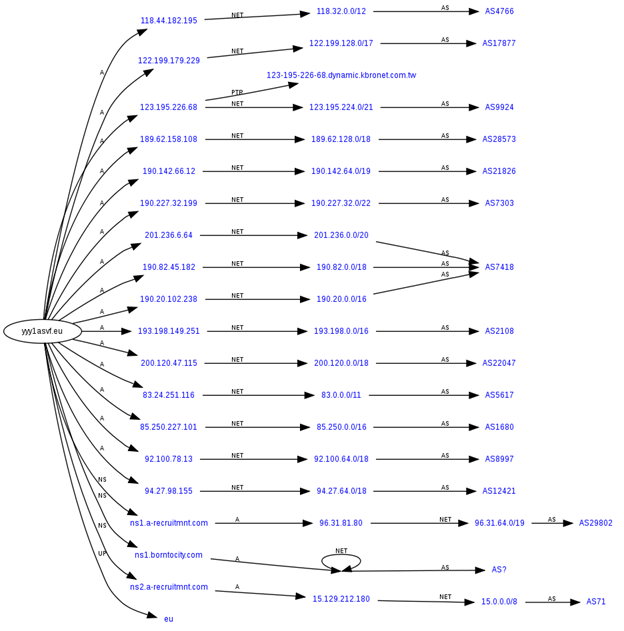
\includegraphics[height=12cm]{./fastflux.png}
  \caption{A visualization of the domain fast-flux. Note the large
  number of IP addresses and domains mapping to a single fully qualified
  domain name used for the C2 server.}
\end{figure}

The above notion presented by the \nsa is idealistic at best in today's climate
of virtually untraceable, anonymous hackers employing robust \dns
techniques such as \textbf{fast flux} \autocite{honey}, which essentially accomplishes hiding a
single \ctwo server by utilizing numerous IP addresses and a
single, rotatable (in an even more difficult-to-trace \textbf{double-flux} methodology)
fully qualified domain name (something as simple as valred.com or hackr.ru, for
example) to very quickly swap between the available IP addresses and \dns records
to avoid detection and backtracing.  Thanks to these particular methods,
problems such as phishing will be omnipresent in the foreseeable future,
exasperated by other countries boasting lax restrictions with regulating the
domain name provisioning.  As such, the NSA’s notion of having organizations
``characterize its adversaries,'' is among the highly impractical and dated points
that weaken the argument for the defense-in-depth strategy.  The only likely
moment adversaries are to be characterized is when it is too late and a network
has already been compromised, such as when the Syrian Electronic Army (SEA)
successfully executed a man-in-the-middle attack rerouting traffic to the U.S.
Marines \autocite{syrians} in 2013.  As such, we keep \scarletshield lightweight and practical
by not addressing this issue; instead, we specifically handle threat prevention
and detection.

Strengths of the defense-in-depth methodology are applied in the implementation
of \scarletshield.  Particularly, one directed focus is on protecting the most
exposed web-facing systems that are typically the target of automated attacks.
This is specifically handled by the robustness of the Snort IDS, which
essentially sniffs all types of Internet Protocol (IP) packets (TCP, UDP, ICMP,
etc.), and checks against patterns, or \emph{rules} and \emph{signatures} indicative of an
attack.  This is reinforced even further by the log-inspection capabilities of
fail2ban, which can essentially pattern-match very common exploits and \dos
traces against typical protocols such as HTTP, SSH, and FTP and react by
blocking IP addresses logged via ``iptables'', a powerful firewall built into most
modern Linux \distros.

Even though iptables comes with modern Linux \distros by default, many end users
beyond actual system and network administrators fail to utilize iptables to its
full potential.  \scarletshield can partly fill the role for a network
administrator when an end user does not have the personnel or resources to fully
utilize iptables themselves.  It can essentially be connected to any switch or
router and be configured to act as a network gateway such that all traffic to
any end user on a network will have to make it past \scarletshield first.

One issue that comes with defense-in-depth is overhead.  How will a user
interface with Snort and fail2ban?  \scarletshield bridges the gap by presenting
all IDS and IPS information and actions in a modern, sleek front-end accessible
via private network (so only computers in the \scarletshield network may access
it) in a way that minimizes the overhead of a network or system administrator
having to manage everything via command line.

In summary, \scarletshield employs a depth of security systems including Snort
and fail2ban while also boasting a breadth of options such as iptables handling
and dropping of malicious sources’ packets while interfacing with other gateways
and subnets to maximize overall security in a network.

\chapter{Approach and Methodology}

As we are designing Scarletshield from scratch with a Ubuntu 12.04 LTS server,
there are several of sub-sections of our Approach and Methodology:

\begin{enumerate}
\item Approach
\item Secure Server SSH
\item Set up of Snort and fail2ban
\item Integration of web front-end
\item Analytics
\item Response Options
\end{enumerate}

\section{Approach}

\scarletshield takes all incoming packets and either accepts or drops them based
on iptables, which is built in to modern Linux \distros such as Ubuntu 12.04 LTS
automatically.  What makes \scarletshield unique is how we deploy an IDS and IPS
through Snort and Fail2ban.  Specifically, IDS mirrors all packets and analyzes
them for patterns (via Snort rules, which are updated every month over the
Internet) indicative of a potential threat, then logging threat signatures on a
database accessible to the administrator and analyzed for new, more strict
iptables rules banning offending IP addresses where necessary.  We utilize
fail2ban to detect obvious brute force, overflows, and exploits in the server
logs (/var/log/auth.log, etc.) to also automatically filter and block IP
addresses preventively, requiring no action from the administrator.

\section{Securing SSH}

Through our research as a group, we came to the conclusion that the safest way
to protect our ssh server against brute forcing would be to change our SSH’s
port from 22 to create security through obscurity.  However, due to the nature
of our research being obscure would not allow us to gather a good pool of log
data.  This led us to a different approach of setting up two factor
authentication.  By utilizing Google’s Google Authenticator API, to successfully
gain access to ScarletShield’s SSH server one must first enter the correct
password, and the unique TOTP security token from RFC6238 generated by the
google authenticator app for the specific user trying to login.  This security
measure makes it impossible for a malicious user to gain login access through
brute fore.

\begin{figure}[h!]
\centering
  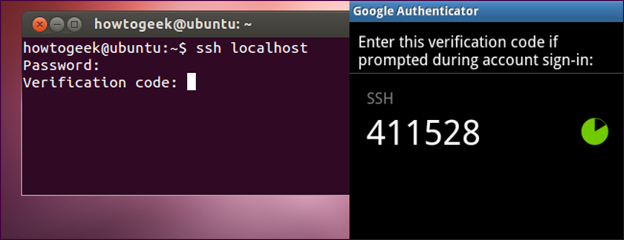
\includegraphics{./goodleauth.png}
  \caption{(Left) A prompt to enter a Google Authenticator verification
  code after typing in a password. (Right) Google Authenticator smart phone application
  generating a verification code.}
\end{figure}

\section{Installation}

Scarletshield covers the breadth of IPS and IDS by implementing both fail2ban
and Snort and interfacing the former with iptables, a user space application for
packet handling.  This not only enables the mobility for a network administrator
to easily be able to monitor incoming traffic and potential threats on a switch,
but also provides an automated mechanism via fail2ban to block obvious, trivial
threats such as brute force attacks and denial-of-service.

Fail2ban is a very simple installation in Ubuntu 12.04 LTS, since it is included
in the advanced packaging tool.  Using its internal mechanism known as ``jails'',
it essentially utilizes filters implemented based on obvious threats (brute
force over SSH, flooding over apache, etc.) and, over a user-set period of time
(default period is several minutes long), bans offending IP addresses for the
duration after it gets caught by Fail2ban via iptables directives packaged with
the program.

Snort is a larger beast with many different variations of configurations
available (types of relational databases used, logging mechanism, etc.); at the
very least, an administrator separately needs to acquire and install libdnet and
the Data Acquisition API \autocite{snort}.  In addition, an administrator must choose a
database and correctly install and configure its respective libraries and server
application.  Due to how fully featured it has become over the years, we chose
MySQL.

\begin{figure}[h]
\centering
  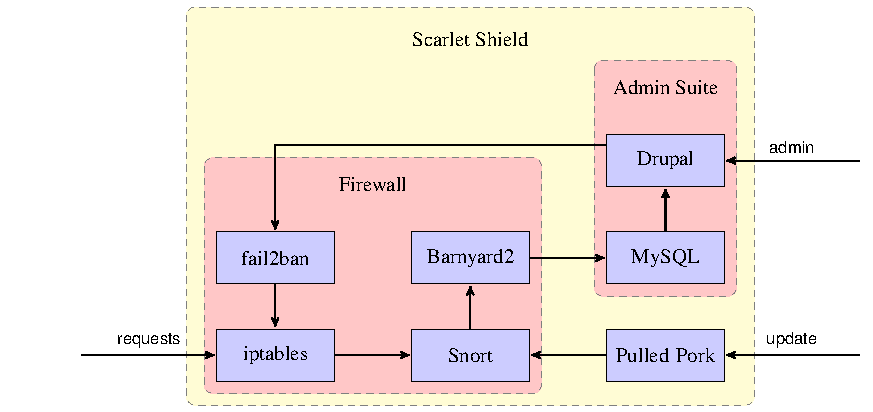
\includegraphics{./scarlet-shield-diagram2.pdf}
  \caption{The architecture of Scarletshield. Incoming packets are routed
  through iptables, where they may be blocked per iptables' rule-set; Snort receives
  the packets and inspects them for signatures of attacks; offending packets are 
  mirrored via Barnyard2 into a MySQL database; users can access the Administrator
  Suite provided by Scarletshield and hosted using Drupal in order to analyze
  attacks against the system; fail2ban automatically bans abusive foreign hosts. 
  Pulled Pork is used to automatically update Snort's classification rulesets
  for offending packet patterns.}
\end{figure}

Once Snort and the database being used are installed, the user must then acquire
and/or update the Snort rule-set, which is essentially how Snort is able to parse
and detect threats within the headers and contents of packets entering the
machine.  We chose ``Pulled Pork'', as it is the most reliable Snort rule management
application, recommended by the creators of Snort themselves.  Finally, the
administrator must interface Snort with the MySQL database.  As of Snort
2.9.3.0, the latest stable version available for Ubuntu 12.04 LTS, it is
required to install the application ``Barnyard2'' for a Snort daemon to record
information into the MySQL database created by a user.

\section{Web Front-end Integration}


Scarletshield features a web frontend utilizing a simple but powerful Drupal
Content Management System (CMS).  In addition, several PHP scripts are
utilized to help analyze and serve the Snort MySQL database.

Scarletshield has three powerful tools for a user that wishes to learn more
about the offending attacks against their server. These three tools, the ``Attack
History'', ``Analytics'' and ``Heatmap'' pages, all come comprise
Scarletshield Suite. Each tool features a different way for the user to view
the logs stored by Scarletshield. The link for the Scarletshield Suite is
\url{http://scarletshield.rutgers.edu/suite}.\footnote{Note that the Scarletshield Suite was
written for the Chrome browser, and some small details will not work on other
browsers.}

When a user tries to access any page of the suite, a JavaScript function runs to
see if the user has an active login cookie with the correct password (the
password is ``scarlet'').  If the user does not have this cookie, they are
redirected to the suite login page seen below.

\begin{figure}[h!]
\centering
  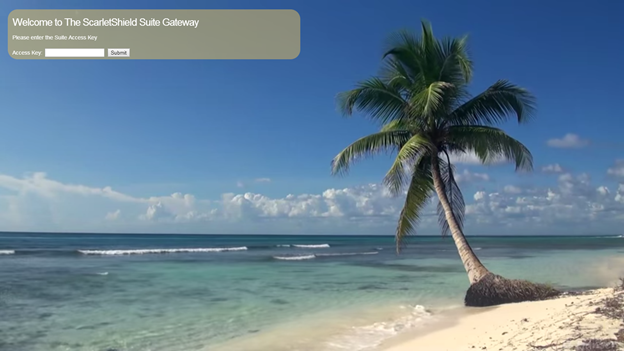
\includegraphics[height=8cm]{./login.png}
  \caption{The Scarletshield Suite login page.}
\end{figure}

The login page makes use of two JQuery packages.  The first package,
``Tubular'', allows a streamed video to be the page background.  The other
package, ``Toastr'', makes use of JavaScript’s non-blocking
architecture.  Toastr is responsible for all asynchronous pop-up alerts.  These
can be seen at page load, and when the access key form's ``Submit'' button is
pressed. Upon entering the correct password, the login cookie is generated and
the user is then brought to the ``Attack History'' page. When first accessing this
page, a loading animation is shown, while the back-end queries data from the MySql
database containing all Snort logs. As a large dataset is loaded from the
server, a screen similar to the one shown below is displayed.

\section{Analytics}

\begin{figure}[h!]
\centering
  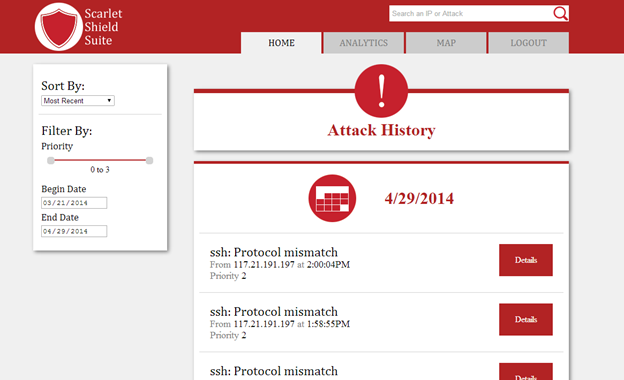
\includegraphics[height=8cm]{./history.png}
  \caption{The Scarletshield Suite Attack History page.}
\end{figure}

Immediately upon visiting the page, the user is given access to all the data
that Snort has logged; the data are logically and visually organized and to
maximize presentability. (For comparison, an early implementation of this
page can be seen here: \url{http://scarletshield.rutgers.edu/demo/last100.php }.) 
Each log is grouped by date and contains information
about the type of attack, the IP address it was originated from, the time it
occurred and the priority of the attack (on a range from 0 to 3 with 0 being
highest priority). If the user presses the ``Details'' button, extra information,
such as the destination IP address (which may not be static if the server has
more than one IP address), the ID number of the occurrence, and approximate
location of the attack are expanded.


\begin{figure}[h!]
\centering
  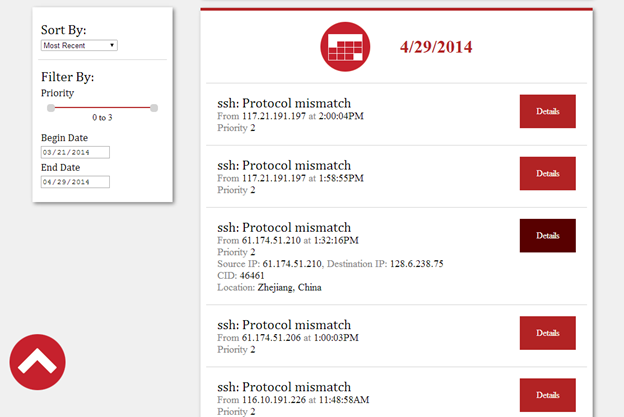
\includegraphics[height=8cm]{./historydet.png}
  \caption{The Scarletshield Suite Attack History page, with an expanded
  description of the details of an attack originating from China.}
\end{figure}

On the top left hand sides of the page, several tools allow the user advanced
filtering capabilities. Logs can be sorted by date (oldest or newest) and
priority (lowest first or highest first), and the search bar at the top can be
used to only show information that either contains the IP address we search or
show attacks that match the string that was searched. This is incredibly
convenient because manually querying for signatures in MySQL (which involves
several tedious SQL joins) would be a time-consuming task for an administrator,
and by having it presented via an admin-accessible private frontend, not only
could administrators react quicker, but even less-skilled users could discover
and report an ongoing attack.

\begin{figure}[h!]
\centering
  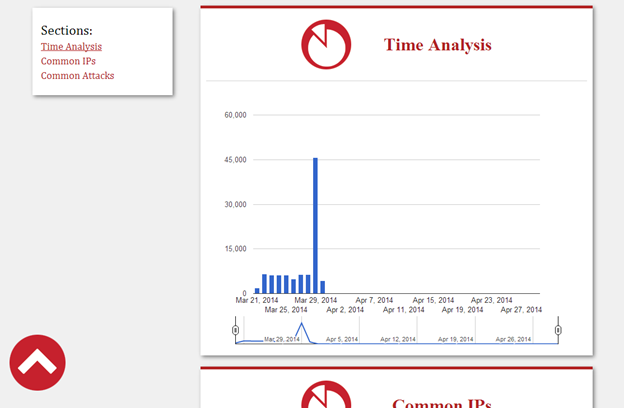
\includegraphics[height=8cm]{./timeanalysis.png}
  \caption{A chart of the rate of attacks over a certain interval. Users
  can use the slider at the bottom of the chart to analyze attacks over
  arbitrary intervals.}
\end{figure}

The Analytics page has three sections, as noted on the sidebar: the “Time
Analysis”, “Common IP’s”, and “Common Attacks”. The Time Analysis section is
simply a chart that shows a chart with the number of attacks that the server has
undergone each day. This chart has a slider to focus on specific time intervals,
and as one can see from the entire view, this is necessary because one single
day may be so active that it dwarfs other days’ activity.


\begin{figure*}[h]
\centering
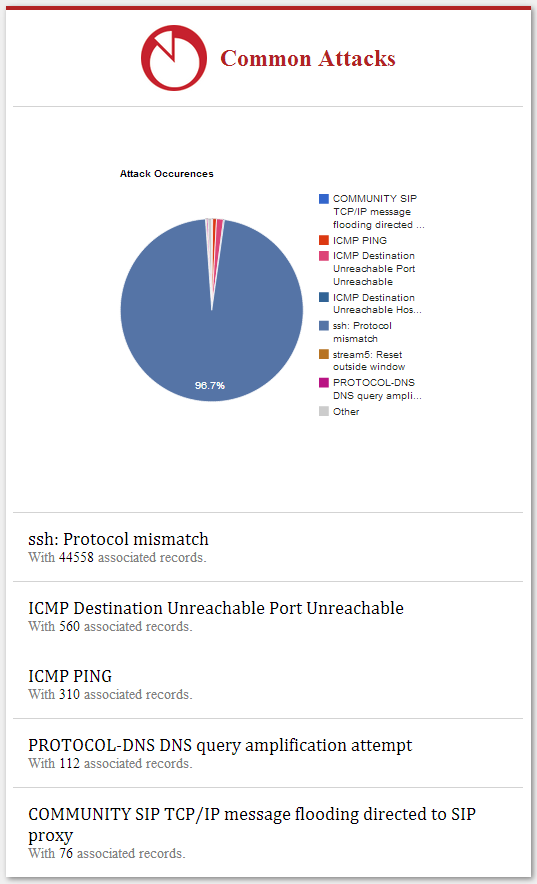
\includegraphics[width=0.45\textwidth]{attackpie.png}\hfill
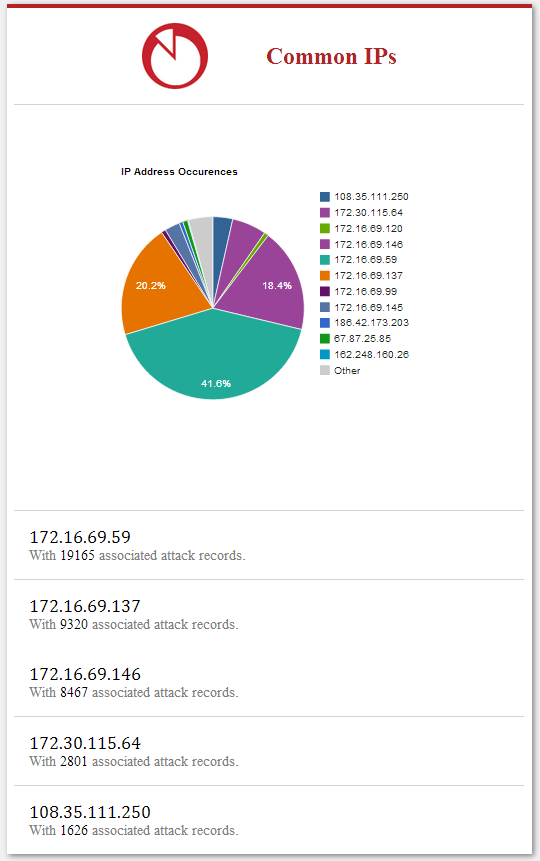
\includegraphics[width=0.45\textwidth]{ippie.png}
\caption{Pie charts featuring prominent attack varieties and IP addresses.}
\end{figure*}

The last page in the Scarletshield Suite is the Heatmap page. Essentially,
Scarlet Shield processes IP addresses from all logged attack patterns and places
it on a Google Map heatmap, so that the user may be able to geographically
backtrace signatures.  In certain configurations, the heatmap would be useful to
backtrace potential ongoing threats and attacks, such as DoS attacks within
certain windows.  This would also help administrators make informed decisions
for creating temporary iptables rules for banning certain offending subnet
servers for the duration of an ongoing threat. An example of the heatmap is
shown below. 

\begin{figure}[h!]
\centering
  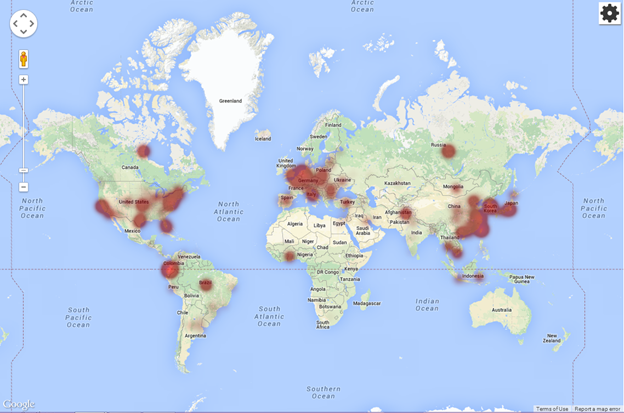
\includegraphics[height=8cm]{./heatmap.png}
  \caption{A geographic world map with red intensity markers indicating
  the presence of attack vectors from a geographic region, identified by IP address.}
\end{figure}

\section{Response Options}

The final portion enabling Scarletshield to cover the full spectrum of network
defense is enabling the network administrator to utilize the frontend for
analysis and decision-making options.  Essentially, the an administrator should
be able to take the Snort records, make an analysis, and decide the action
(whether to throttle or drop all packets altogether from a suspicious IP
address) to take to ensure network security.

Due to time constraints, this feature was not integrated into the administrator
suite, although the capability is already inherently present because of the
inclusion of fail2ban. Future work could easily incorporate the addition of such
an administrator response suite.

\chapter{Conclusion}

During this semester, we achieved the following goals:

\begin{enumerate}
\item Deployed a Ubuntu 12.04 LTS server with Apache, MySQL, Php, Drupal, Snort,
		Pulled Pork, Barnyard2, fail2ban, and integrated them with iptables
\item Configured Snort to update via Pulled Pork and to log to MySQL via Barnyard2
\item Established initial rules and filters for Snort and Fail2ban
\item Utilized PHP scripts to build monitoring and analysis suite into Drupal
\item Provided dynamic and user-friendly analytics charting and mapping tools
\end{enumerate}

Overall, we’ve made great strides in rounding out the backend for Scarletshield; 
we additionally have the basic framework established for Scarletshield, with a 
good number of scripts and visualization tools to assist a network administrator.

\section{Future Work}

Although Scarletshield is already operational on a server within Rutgers
Engineering, additional work is necessary to integrate it into private subnets
and to give it world-wide-web scale. More robustness and failover capabilities
are needed in order to communicate certain threats that may be large-scale, and
which would otherwise disrupt significant cybersecurity infrastructure. This
also requires fine tuning Scarletshield’s frontend capabilities and adding more
analysis tools and automation techniques to streamline the threat-analysis and
threat-prevention workflow presented to the network administrator.  Further
integration of the subcomponents of Scarletshield will solidify its versatility,
relevance, and overall strength.  By successfully implementing a fully-featured
frontend for monitoring and reacting to threats, we will maximize the potential
of Scarletshield to be deployable to both private switches and enterprise-level
networks.

Primarily, this entails better integrating current monitoring scripts with
Drupal.

Moving forward we envision multiple ScarletShield deployments being used to
protect a multitude of systems simultaneously.  With this in mind we plan on
creating a global set of black lists and logs that all deployments can
access and update.  Maintaining global lists would allow each individual
deployment of ScarletShield to share collective knowledge. If one instance
of ScarletShield is attacked, another deployment can preemptively block the
attacker instead of waiting to be attacked itself.

Also, our scripts will allow administrators the option to take action on
addresses logged with signatures, along with varying degrees of reaction
steps they may be able to take (functionality to throttle or ban IPs
altogether, for example), such that Scarletshield will give full control to
the network administrator.

Additionally, we will be working on a way to replicate the Scarletshield
build; this will most likely be accomplished by presenting a ISO image that
can be installed in managed switch servers.


%\begin{figure*}[t]
%\centering
%\subfloat[\textrm{g = [0 0 0 0 0 0 0 0]}]{\label{part2a}
%\includegraphics[width=0.4\textwidth]{./pics/part2a.png}}\hfill
%\subfloat[\textrm{g = [8 6 2 0 0 1 3 6]}]{\label{part2b}
%\includegraphics[width=0.4\textwidth]{./pics/part2b.png}}\\
%\subfloat[\textrm{g = [-10 -10 -10 -10 10 -10 -10 -10]}]{\label{part2c}
%\includegraphics[width=0.4\textwidth]{./pics/part2c.png}}\hfill
%\subfloat[\textrm{g = [-3 -2 -1 2 2 -3 -5 8]}]{\label{part2d}
%\includegraphics[width=0.4\textwidth]{./pics/part2d.png}}
%\label{fig:part2}
%\caption{Sample frequency band gain values.}
%\end{figure*}

\printbibliography

\end{document}